\documentclass[9pt,twoside]{extarticle}
\usepackage[a5paper, vmargin=0.35in, hmargin=0.65in, includefoot]{geometry}
\usepackage[utf8]{inputenc}

\usepackage[skip=12pt]{parskip}

\usepackage{titlesec}
\newcommand{\sectionbreak}{\clearpage}
\titleformat{\section}{\normalfont\fontsize{12}{18}\bfseries\filcenter}{\thesection}{0em}{}
\titlespacing{\section}{0pt}{40pt}{30pt}

\titleformat{\subsection}{\normalfont\fontsize{10}{14}\bfseries\filcenter}{\thesubsection}{0em}{}
\titlespacing{\section}{0pt}{30pt}{20pt}

\titleformat{\subsubsection}{\normalfont\fontsize{10}{14}\bfseries\filcenter}{\thesubsubsection}{0em}{}
\titlespacing{\section}{0pt}{20pt}{10pt}

\usepackage{ifthen}
\usepackage{xcolor}

\usepackage{tgpagella}
\usepackage{mathpazo}

\usepackage{verse}
\setlength{\leftmargini}{0em}

\usepackage{tocloft}
\renewcommand\cftsecfont{\mdseries}
\usepackage{hyperref}
% \renewcommand{\cftsecleader}{\cftdotfill{\cftdotsep}} % for sections, if you really want! (It is default in report and book class (So you may not need it).

\usepackage{fancyhdr}
\fancyhf{} % clear all header and footers
\renewcommand{\headrulewidth}{0pt} % remove the header rule
\fancyfoot[LO,RE]{\thepage} % Left side on Even pages; Right side on Odd pages
\pagestyle{fancy}
\fancypagestyle{plain}{
  \fancyhf{}
  \renewcommand{\headrulewidth}{0pt}
  \fancyhf[lef,rof]{\thepage}
}

\setcounter{secnumdepth}{0} % sections are level 1

\usepackage{qrcode}

\usepackage{graphicx}

%%%%%%%%%%%%%%%%%%%%%%%%%%%%%%%%%%%%%%%%%%%%%%%%%%%%%%%%%%%%%%%%%%%%%%%%%%%%%%%%

\newenvironment{xverse}{
	\begin{verse}
	\fontsize{8.5}{10.5}\selectfont
	}
	{
	\end{verse}
	\penalty 0
}
\newcommand{\chorusdef}{\textbf{\emph{Chorus:}}\\*}
\setlength{\stanzaskip}{10pt}
\newcommand{\chorusmark}[1][1]{%
\vspace{-0.5\stanzaskip}%
\textbf{\emph{Chorus \ifthenelse{\equal{#1}{1}}{}{$\times$ #1}}}%
\vspace{-0.5\stanzaskip}%
}
\newcommand{\gray}[1]{\textcolor{gray}{#1}}

\title{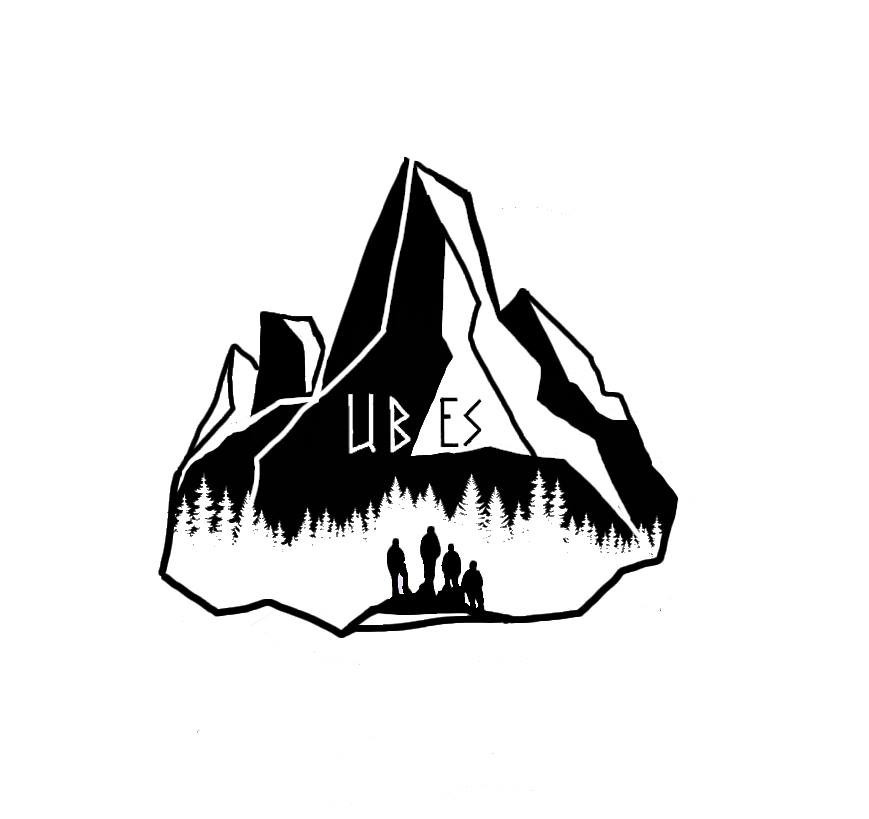
\includegraphics[width=0.6\textwidth]{logo.jpg}\\UBES Songbook}
\author{Prototype 0.4}
\date{2019 - 2020}

\begin{document}
\raggedbottom
\pagenumbering{gobble}


\maketitle
\newpage

\section*{Foreword}

\subsection*{Acknowledgements}

\begin{center}
Special thanks to Alice Denning for collecting these songs -- she did the hard
work to make this happen.

Special thanks to Charlie Harding for large amounts of work editing and
typesetting the songs.
\end{center}

\subsection*{Music}
\begin{center}

Playlists for the songbook, for various streaming services. The QR codes are
clickable if you have the pdf.

\subsubsection*{Spotify}
\quad
\qrcode[height=1.6in]{https://open.spotify.com/playlist/2a8qmHglthbuB5US3cEcuU}
\subsubsection*{Youtube}
\quad
\qrcode[height=1.6in]{https://music.youtube.com/playlist?list=PLp4mBwNJeO-zGOchjv0GJUi5-3BZGbi7F}


\end{center}
\newpage

\tableofcontents

\sectionbreak
\pagenumbering{arabic}

\section{Bones in the Ocean}
\begin{xverse}
Oh, I bid farewell to the port and the land, \\*
And I paddle away from brave England’s white sands, \\*
To search for my long ago forgotten friends, \\*
To search for the place I hear all sailors end.

As the souls of the dead fill the space of my mind, \\*
I’ll search without sleeping till peace I can find. \\*
I fear not the weather, I fear not the sea, \\*
I remember the fallen, do they think of me? \\*
When their bones in the ocean forever will be.

Plot a course through the night to a place I once knew, \\*
To a place where my hope died along with my crew. \\*
So I swallow my grief and face life’s final test: \\*
To find promise of peace and the solace of rest.

As the songs of the dead fill the space of my ears, \\*
Their laughter like children, their beckoning cheers, \\*
My heart longs to join them, sing songs of the sea, \\*
I remember the fallen, do they think of me? \\*
When their bones in the ocean forever will be.

When at last before my ghostly shipmates I stand, \\*
I shed a small tear for my home upon land. \\*
Though their eyes speak of depths filled with struggle and strife, \\*
Their smiles below say I don’t owe them my life.

As the souls of the dead fill the space of my eyes, \\*
And my boat listed over and tried to capsize, \\*
I’m this far from drowning, this far from the sea, \\*
I remember the living do they think of me? \\*
When my bones in the ocean forever will be.

Now that I’m staring down at the darkest abyss, \\*
I’m not sure what I want but I don’t think it’s this. \\*
As my comrades call to stand fast and forge on, \\*
I make sail for the dawn till the darkness has gone.

As the souls of the dead live fore’er in my mind, \\*
As I live all the years that they left me behind, \\*
I’ll stay on the shore but still gaze at the sea, \\*
I remember the fallen and they think of me, \\*
For our souls in the ocean together will be.

I remember the fallen and they think of me, \\*
For our souls in the ocean together will be.
\end{xverse}

\section{Santiana}
\begin{xverse}
Oh Santiana gained the day! \\*
Away Santiana! \\*
Napoleon of the West, they say! \\*
Along the plains of Mexico.

\chorusdef
Well heave her up and away we’ll go, \\*
Away, Santiana! \\*
Heave her up and away we’ll go, \\*
Along the plains of Mexico.

She’s a fast clipper ship and a bully good crew: \\*
Away, Santiana! \\*
And an old salty Yank for a captain too, \\*
Along the plains of Mexico.

\chorusmark

Santiana fought for gold, \\*
Away, Santiana! \\*
Around Cape Horn through the ice and snow, \\*
Along the plains of Mexico.

\chorusmark

’Twas on the field of Molley-Del-Rey, \\*
Away, Santiana! \\*
Well both his legs got blown away, \\*
Along the plains of Mexico.

\chorusmark

It was a fierce and bitter strife, \\*
Away, Santiana! \\*
The general Taylor took his life, \\*
Along the plains of Mexico.

\chorusmark

Santiana now we mourn, \\*
Away, Santiana! \\*
We left him buried off Cape Horn, \\*
Along the plains of Mexico.
\end{xverse}


\section{Loch Lomond}

\begin{xverse}
By yon bonnie banks and by yon bonnie braes, \\*
Where the sun shines bright on Loch Lomond, \\*
Where me and my true love were e’er wont to gae, \\*
In the bonnie, bonnie banks of Loch Lomond.

\chorusdef
O ye’ll take the high road, and I’ll take the low road, \\*
And I’ll be in Scotland afore ye, \\*
Where me and my true love will never meet again, \\*
On the bonnie, bonnie banks of Loch Lomond.

’Twas there that we parted, in yon shady glen, \\*
On the steep, steep side o’ Ben Lomond, \\*
Where, deep in the purple hue, the highland hills we view, \\*
And the moon coming out in the gloaming.

\chorusmark

The wee birdies sing and the wild flowers spring, \\*
And in sunshine the waters lie sleeping. \\*
But the broken heart it kens nae second spring again, \\*
Though the waeful may cease frae their grieving.

\chorusmark
\end{xverse}

\section{Beeswing}
\begin{xverse}
I was 18 when I came to town, they called it the Summer of Love: \\*
Burning babies, burning flags, the Hawks against the Doves. \\*
I took a job at the steaming way down on Cauldrum Street, \\*
Fell in love with a laundry girl that was workin’ next to me.

\chorusdef
She was a rare thing fine, as a bee’s wing, \\*
So fine a breath of wind might blow her away. \\*
She was a lost child, she was runnin’ wild (she said) \\*
She said, “As long as there’s no price on love, I’ll stay, \\*
And you wouldn’t want me any other way.”

Brown hair zig-zag around her face, and a look of half-surprise \\*
Like a fox caught in the headlights, there was animal in her eyes. \\*
She said, “Young man, oh can’t you see, I’m not the factory kind; \\*
If you don’t take me out of here, I’ll surely lose my mind."

\chorusmark

We busked around the market towns and picked fruit down in Kent \\*
And we could tinker pots and pans and knives wherever we went. \\*
I said to her we’ll settle down, get a few acres dug, \\*
A fire burning in the hearth and babies on the rug. \\*
She said, “Oh man, you foolish man, that surely sounds like hell, \\*
You might be lord of half the world, you’ll not own me as well.”

\chorusmark

We was camping down the Gower one time, The work was pretty good \\*
She thought we shouldn’t wait for the frost, and I thought maybe we should; \\*
We was drinking more in those days, and tempers reached a pitch, \\*
And like a fool I let her run with the rambling itch.

Oh the last I heard she’s sleeping rough back on the Derby beat, \\*
White Horse in her hip pocket, and a wolfhound at her feet, \\*
And they say she even married once, a man named Romany Brown, \\*
But even a gypsy caravan was too much settling down. \\*
And they say her flower is faded now, hard weather and hard booze, \\*
But maybe that’s just the price you pay for the chains you refuse

She was a rare thing, fine as a bee’s wing \\*
I miss her more than ever words can say \\*
If I could just taste all of her wildness now \\*
If I could hold her in my arms today… \\*
I wouldn’t want her any other way
\end{xverse}

\section{Leave her, Johnny}

\begin{xverse}
I thought I heard the Old Man say: \\*
“Leave her, Johnny, leave her.” \\*
Tomorrow you will get your pay, \\*
And it’s time for us to leave her.

\chorusdef
Leave her, Johnny, leave her! \\*
Oh, leave her, Johnny, leave her! \\*
For the voyage is long and the winds don’t blow, \\*
And it’s time for us to leave her.

Oh, the wind was foul and the sea ran high; \\*
“Leave her, Johnny, leave her!” \\*
She shipped it green and none went by, \\*
And it’s time for us to leave her.

\chorusmark

I hate to sail on this rotten tub; \\*
“Leave her, Johnny, leave her!” \\*
No grog allowed and rotten grub, \\*
And it’s time for us to leave her.

\chorusmark

We swear by rote for want of more; \\*
“Leave her, Johnny, leave her!” \\*
But now we’re through so we’ll go on shore, \\*
And it’s time for us to leave her.

\chorusmark
\end{xverse}

\section{Northwest Passage}

\begin{xverse}
\chorusdef
Ah, for just one time, \\*
I would take the Northwest Passage \\*
To find the hand of Franklin \\*
Reaching for the Beaufort Sea; \\*
Tracing one warm line \\*
Through a land so wild and savage, \\*
And make a Northwest Passage to the sea.

Westward from the Davis Strait \\*
’Tis there ’twas said to lie: \\*
The sea route to the Orient \\*
For which so many died. \\*
Seeking gold and glory, \\*
Leaving weathered, broken bones, \\*
And a long-forgotten lonely cairn of stones.

\chorusmark

Three centuries thereafter \\*
I take passage overland, \\*
In the footsteps of brave Kelso \\*
Where his “sea of flowers” began. \\*
Watching cities rise before me \\*
Then behind me sink again, \\*
This tardiest explorer \\*
Driving hard across the plain.

\chorusmark

And through the night, behind the wheel, \\*
The mileage clicking west, \\*
I think upon Mackenzie, \\*
David Thompson and the rest, \\*
Who cracked the mountain ramparts \\*
And did show a path for me, \\*
To race the roaring Fraser to the sea

\chorusmark

How then am I so different \\*
From the first men through this way? \\*
Like them, I left a settled life, \\*
I threw it all away! \\*
To seek a Northwest Passage, \\*
At the call of many men, \\*
To find there but the road back home again.

\chorusmark
\end{xverse}

\section{The Mingulay Boat Song}

\begin{xverse}
\chorusdef
Heave ’er ho, boys; let her go, boys; \\*
Swing her head round, into the weather. \\*
Heave ’er ho, boys; let her go, boys; \\*
Sailing homeward to Mingulay. \\*

What care we though, white the Minch is? \\*
What care we, boys, for windy weather? \\*
When we know that every inch is \\*
Sailing homeward to Mingulay

\chorusmark

Wives are waiting, by the pierhead, \\*
Gazing seaward, from the heather, \\*
Bring ahead ’round, boys, then we’ll anchor, \\*
Ere the sun sets on Mingulay.

\chorusmark

Ships return now, heavy laden, \\*
Mothers holdin’ bairns a-cryin’. \\*
They’ll return, yet, when the sun sets, \\*
Sailing homeward to Mingulay.

\chorusmark[2]
\end{xverse}

\section{The Skye Boat Song}

\begin{xverse}
\chorusdef
Speed, bonnie boat, like a bird on the wing, \\*
Onward! the sailors cry; \\*
Carry the lad that’s born to be King \\*
Over the sea to Skye.

Loud the winds howls, loud the waves roar, \\*
Thunderclaps rend the air; \\*
Baffled, our foes stand by the shore, \\*
Follow they will not dare.

\chorusmark

Many’s the lad, fought on that day \\*
Well the claymore did wield; \\*
When the night came, silently lay \\*
Dead on Culloden’s field.

\chorusmark

Though the waves leap, soft shall ye sleep, \\*
Ocean’s a royal bed. \\*
Rocked in the deep, Flora will keep \\*
Watch by your weary head. \\*

\chorusmark
\end{xverse}

\section{Wild Mountain Thyme (Will Ye Go, Lassie, Go?)}

\begin{xverse}
O the summer time has come, \\*
And the trees are sweetly bloomin’, \\*
And the wild mountain thyme, \\*
Grows around the bloomin’ heather. \\*
Will ye go, Lassie, go?

\chorusdef
And we’ll all go together, \\*
To pull wild mountain thyme, \\*
All around the bloomin’ heather, \\*
Will ye go, Lassie, go?

I will build my love a bower, \\*
By yon cool crystal fountain. \\*
And round it I will pile \\*
All the wild flowers o’ the mountain. \\*
Will ye go, Lassie, go?

\chorusmark

I will range through the wilds, \\*
And the deep glen sae dreamy, \\*
And return wi’ their spoils, \\*
Tae the bower o’ my dearie. \\*
Will ye go, Lassie, go?

\chorusmark

If my true love she’ll not come, \\*
Then I’ll surely find another, \\*
To pull wild mountain thyme, \\*
All around the bloomin’ heather. \\*
Will ye go, Lassie, go?

\chorusmark
\end{xverse}

\section{The Wild Rover}

\begin{xverse}
I’ve been a wild rover for many’s the year, \\*
And I’ve spent all me money on whiskey and beer. \\*
But now I’m returning with gold in great store, \\*
And I never will play the wild rover no more

\chorusdef
And it’s no, nay, never, \\*
No, nay, never no more, \\*
Will I play the wild rover, \\*
No, never no more!

I went into an alehouse I used to frequent, \\*
And I told the landlady me money was spent, \\*
I asked her for credit, she answered me, “Nay! \\*
Such a custom as yours I can have any day.”

\chorusmark

I then took from me pocket ten sovereigns bright, \\*
And the landlady’s eyes opened wide with delight, \\*
She says, “I have whiskeys and wines of the best, \\*
And the words that you told me were only in jest.”

\chorusmark

I’ll go home to my parents, confess what I’d done, \\*
And I’ll ask them to pardon their prodigal son, \\*
And when they’ve caressed me as ofttimes before, \\*
I never will play the wild rover no more.

\chorusmark[2]
\end{xverse}

\section{Caledonia}

\begin{xverse}
I don’t know if you can see, \\*
The changes that have come over me: \\*
In these last few days I’ve been afraid \\*
That I might drift away. \\*
So I’ve been telling old stories, singing songs \\*
that make me think about where I come from, \\*
And that’s the reason why I seem so far away today.

\chorusdef
Oh and let me tell you that I love you, \\*
And I think about you all the time: \\*
Caledonia, you’re calling me and now I’m going home. \\*
If I should become a stranger, \\*
You know that it would make me more than sad: \\*
Caledonia’s been everything I’ve ever had.

I have moved and I’ve kept on moving, \\*
Proved the points that I needed proving. \\*
Lost the friends that I needed losing, \\*
Found others on the way. \\*
I have tried and I’ve kept on trying, \\*
Stolen dreams, yes there’s no denying. \\*
I have travelled hard, with my conscience flying, \\*
Somewhere with the wind.

\chorusmark

Now I’m sitting here before the fire, \\*
The empty room, the forest choir. \\*
The flames that couldn’t get any higher, \\*
They’ve withered now they’ve gone. \\*
But I’m steady thinking, my way is clear, \\*
And I know what I will do tomorrow: \\*
When the hands have shaken and the kisses flowed, \\*
Then I will disappear.

\chorusmark
\end{xverse}

\section{Whiskey in the Jar}

\begin{xverse}
As I was a goin’ over the far-famed Kerry Mountains, \\*
I met with Captain Farrell, and his money he was countin’. \\*
I first produced my pistol and I then produced my rapier, \\*
sayin’, “Stand and deliver for I am your bold deceiver”:

\chorusdef
Mush-a ring dum-a do dum-a da; \gray{(4 claps)} \\*
Whack for the daddy-o; \gray{(2 claps)} \\*
Whack for the daddy-o; \\*
There’s whiskey in the jar! \gray{(yell “HEY” with a simultaneous clap)}

I counted up my money and it made a pretty penny. \\*
I took that money home and I took it home Jenny; \\*
She sighed and she swore that she never would deceive me, \\*
But the devil take the women, for they never can be easy:

\chorusmark

I went into my chamber, all for to take a slumber, \\*
I dreamt of gold and jewels and for sure ’twas no wonder. \\*
But Jenny took my charges and filled them up with water, \\*
And sent for Captain Farrell to be ready for the slaughter:

\chorusmark

’Twas early in the mornin’ before I rose to travel; \\*
Up comes a band of footmen and likewise captain Farrell. \\*
I first produced me pistol for she stole away me rapier; \\*
I couldn’t shoot the water, so a prisoner I was taken.

\chorusmark

If anyone can aid me, ’tis my brother in the army, \\*
If I can find his station in Cork or in Killarney, \\*
And if he’ll go with me, we’ll go rovin’ through Killkenny, \\*
And I’m sure he’ll treat me better than my own a-sporting Jenny!

\chorusmark

\chorusmark
\end{xverse}
\section{Rocky Road to Dublin}

\begin{xverse}
In the merry month of June, when from my home I started, \\*
Left the girls of Tuam nearly broken-hearted. \\*
Saluted Father dear, kissed my darling mother, \\*
Drank a pint of beer, my grief and tears to smother; \\*
Then off to reap the corn, leave where I was born, \\*
Cut a stout black-thorn to banish ghosts and goblins; \\*
Brand new pair of brogues, rattlin’ o’er the bogs, \\*
Frightenin’ all the dogs on the rocky road to Dublin, \\*
One, two, three, four, five!

\chorusdef
Hunt the hare and turn her down the rocky road \\*
And all the way to Dublin, whack, follol le-rah!

In Mullingar, that night, I rested, limbs so weary. \\*
Started by daylight, my spirits bright and airy; \\*
Took a drop of pure, keep me heart from sinking; \\*
That’s the Paddy’s cure, whene’er he’s on for drinking, \\*
To see the lassies smile, laughing all the while, \\*
At me curious style, ’twould set your heart a-bubblin’ \\*
An’ asked me was I hired, wages I required, \\*
’Til I was nearly tired of the rocky road to Dublin, \\*
One, two, three, four, five!

\chorusmark

In Dublin next arrived, I thought it such a pity, \\*
To be so soon deprived a view of that fine city. \\*
So then I took a stroll, all among the quality; \\*
Bundle it was stole, all in a neat locality \\*
Something crossed me mind, when I looked behind \\*
No bundle could I find upon me stick a-wobblin’. \\*
Enquiring after the rogue, said me Connaught brogue \\*
Wasn’t much in vogue on the rocky road to Dublin, \\*
One, two, three, four, five!

\chorusmark

From there I got away, me spirits never falling. \\*
Landed on the quay, just as the ship was sailing. \\*
The Captain at me roared, said that no room had he; \\*
When I jumped aboard, a cabin found for Paddy \\*
Down among the pigs, played some hearty jigs, \\*
Danced some hearty rigs, the water round me bubbling; \\*
When off Holyhead I wished meself was dead \\*
Or better far instead, on the rocky road to Dublin, \\*
One, two, three, four, five!

\chorusmark

The boys of Liverpool, when we safely landed \\*
Called meself a fool, I could no longer stand it: \\*
Blood began to boil, temper I was losing; \\*
Poor old Erin’s Isle they began abusing. \\*
“Hurrah me soul!” says I, me \emph{shillelagh} I let fly, \\*
Some Galway boys were nigh and saw I was a-hobblin’. \\*
With a loud “hurray!” they joined in the affray, \\*
Quickly cleared the way for the rocky road to Dublin, \\*
One, two, three, four, five!

\chorusmark[2]
\end{xverse}


\section{Retirement Song}

\begin{xverse}
I’ve been roaming all my life, \\*
And now I’ve found a lady wife, \\*
I’m staying, right here. \\*
Oh, I won’t go sailing anymore, \\*
I won’t obey the oceans call, \\*
I’m staying right here.

\chorusdef
I’ll be a man of the land, \\*
I’ll be a man of the trees, \\*
I’ll be a man, wherever my woman will be. \\*
I won’t be any captains mate, \\*
I won’t be servant of the seas; \\*
’Cause this pretty little woman is all I need.

At 14 I was cabin boy \\*
To fearsome Captain Buckleroy, \\*
I’m staying right here. \\*
When I was sick he ordered cat-a-nine, \\*
Until I said that I felt fine, \\*
I’m staying right here,

\chorusmark

At 20 I manned that crow’s nest \\*
And captain said “I was the best”, \\*
I’m staying right here, \\*
But I nearly lost my eyes to god, \\*
Just looking out for old cape cod, \\*
I’m staying right here.

\chorusmark

At 25 no man alive \\*
Could match my skills for gun’en, \\*
I’m staying right here, \\*
But the Captain he got drunk one night \\*
And sank the blasted cannon, \\*
I’m staying right here,

\chorusmark

Captain died at 28 \\*
And by then I was his first mate, \\*
I’m staying right here \\*
Oh they tried to give me his command \\*
But I was hungry for the land, \\*
I’m staying right here,

\chorusmark

Stepped ashore at Felixstowe \\*
And made for Bristol by the road, \\*
I’m staying right here, \\*
Well I fell in love, when, first, I saw, her, \\*
Avon county’s finest daughter, \\*
And now she’s got me staying right here, \\*
Hoo-hey!

\chorusmark

I’ll be a man of the land, \\*
I’ll be a man of the trees, \\*
I’ll be a man, wherever my woman will be. \\*
I won’t be any captains mate, \\*
I won’t be servant of the seas; \\*
’Cause this pretty, little, woman, is, all, I, need.
\end{xverse}

\section{The Parting Glass}

\begin{xverse}
Of all the money that e’er I had \\*
I spent it in good company \\*
And all the harm I’ve ever done \\*
Alas, it was to none but me \\*
And all I’ve done for want of wit \\*
To memory now I can’t recall \\*
So fill to me the parting glass \\*
Good night and joy be to you all

So fill to me the parting glass \\*
And drink a health whate’er befalls \\*
Then gently rise and softly call \\*
“Good night and joy be to you all”

Of all the comrades that e’er I had \\*
They’re sorry for my going away \\*
And all the sweethearts that e’er I had \\*
They’d wish me one more day to stay

But since it fell into my lot \\*
That I should rise and you should not \\*
I’ll gently rise and softly call \\*
“Good night and joy be to you all”

But since it fell into my lot \\*
That I should rise and you should not \\*
I’ll gently rise and softly call \\*
“Good night and joy be to you all”

So fill to me the parting glass \\*
And drink a health whate’er befalls \\*
Then gently rise and softly call \\*
“Good night and joy be to you all” \\*
Good night and joy be to you all
\end{xverse}

\section{Spanish Ladies}

\begin{xverse}
Farewell and adieu to you Spanish Ladies, \\*
Farewell and adieu to you ladies of Spain; \\*
For we’ve received orders for to sail for old England, \\*
But we hope very soon that we’ll see you again!

\chorusdef
We’ll rant and we’ll roar, like true British sailors, \\*
We’ll rant and we’ll roar, all on the salt seas, \\*
Until we strike soundings in the channel of old England; \\*
From Ushant to Scilly is thirty-five leagues.
 
We hove our ship to with the wind from sou’west, boys, \\*
We hove our ship to, our soundings to see; \\*
We rounded and sounded, got fourty five fathoms, \\*
Then we squared our main yard and up channel steered we.

\chorusmark

The first land we sighted was callèd the Dodman, \\*
Next Rame Head off Plymouth, Start, Portland and Wight; \\*
We sailed by Beachy, by Fairlight and Dover \\*
And then we bore up for the South Foreland light

\chorusmark

Then the signal was made for the grand fleet to anchor, \\*
And all in the Downs that night for to lie; \\*
Then it's stand by your stoppers, steer clear your shank-painters, \\*
Haul up your clew garnets, let tacks and sheets fly!

\chorusmark

So let every man toss off a full bumper, \\*
and let every man drink up a full glass; \\*
We'll drink and be merry and drown melancholy, \\*
singing here's a good health to each true-hearted lass!

\chorusmark
\end{xverse}

\section{Seven Drunken Nights}

\begin{xverse}
Oh, as I went home on Monday night, \\*
As drunk as drunk could be, \\*
I saw a horse outside the door, \\*
Where my old horse should be. \\*
Well, I called me wife and I said to her, \\*
“Will you kindly tell to me, \\*
Who owns that horse outside the door, \\*
Where my old horse should be?” \\*
\textit{Aye, you’re drunk, you’re drunk, you silly old fool, \\*
Still you cannot see: \\*
That’s a lovely sow that my mother sent to me!} \\*
Well, it’s many a day I’ve travelled, a hundred miles or more, \\*
But a saddle on a sow, sure, I never saw before!

And as I went home on Tuesday night, \\*
As drunk as drunk could be, \\*
I saw a coat behind the door, \\*
Where my old coat should be. \\*
Well, I called me wife and I said to her, \\*
“Will you kindly tell to me: \\*
Who owns that coat behind the door, \\*
Where my old coat should be?” \\*
\textit{Aye, you’re drunk, you’re drunk, you silly old fool, \\*
Still you cannot see: \\*
That’s a woollen blanket that me mother sent to me!} \\*
Well, it’s many a day I’ve travelled, a hundred miles or more, \\*
But buttons on a blanket, sure, I never saw before!

And as I went home on Wednesday night, \\*
As drunk as drunk could be, \\*
I saw a pipe upon the chair, \\*
Where my old pipe should be. \\*
Well, I called my wife and I said to her, \\*
“Will you kindly tell to me: \\*
Who owns that pipe upon the chair, \\*
Where my old pipe should be?” \\*
\textit{Aye, you’re drunk, you’re drunk, you silly old fool, \\*
Still you cannot see: \\*
That’s a lovely tin-whistle, that me mother sent to me!} \\*
Well, it’s many a day I’ve travelled, a hundred miles or more, \\*
But tobacco in a tin-whistle, sure, I never saw before!

And I went home on Thursday night, \\*
As drunk as drunk could be, \\*
I saw two boots beneath the bed, \\*
Where my old boots should be. \\*
Well, I called me wife and I said to her, \\*
“Will you kindly tell to me: \\*
Who owns them boots beneath the bed, \\*
Where my old boots should be?” \\*
\textit{Aye, you’re drunk, you’re drunk, you silly old fool, \\*
Still you cannot see: \\*
They’re two lovely geranium pots me mother sent to me!} \\*
Well, it’s many a day I’ve travelled, a hundred miles or more, \\*
But laces in geranium pots I never saw before!

And as I came home on Friday night, \\*
As drunk as drunk could be, \\*
I saw a head upon the bed, \\*
Where my old head should be. \\*
Well, I called my wife and I said to her, \\*
“Will you kindly tell to me: \\*
Who owns that head upon the bed, \\*
Where my old head should be?” \\*
\textit{Aye, you’re drunk, you’re drunk, you silly old fool, \\*
Still you cannot see: \\*
That’s a baby boy that me mother sent to me!} \\*
Well, it’s many a day I’ve travelled, a hundred miles or more, \\*
But a baby boy with his whiskers on, sure, I never saw before!
\end{xverse}

\section{Barrett’s Privateers}

\begin{xverse}
Oh, the year was 1778 \\*
How I wish I was in Sherbrooke now \\*
A letter of marque came from the king \\*
To the scummiest vessel I’ve ever seen \\*
God damn them all! I was told \\*
We’d cruise the seas for American gold \\*
We’d fire no guns, shed no tears \\*
But I’m a broken man on a Halifax pier \\*
The last of Barrett’s Privateers

Oh, Elcid Barrett cried the town \\*
How I wish I was in Sherbrooke now \\*
For twenty brave men all fishermen who \\*
Would make for him the Antelope’s crew \\*
God damn them all! I was told \\*
We’d cruise the seas for American gold \\*
We’d fire no guns, shed no tears \\*
But I’m a broken man on a Halifax pier \\*
The last of Barrett’s Privateers

The Antelope sloop was a sickening sight \\*
How I wish I was in Sherbrooke now \\*
She’d a list to the port and her sails in rags \\*
And the cook in the scuppers with the staggers and jags \\*
God damn them all! I was told \\*
We’d cruise the seas for American gold \\*
We’d fire no guns, shed no tears \\*
But I’m a broken man on a Halifax pier \\*
The last of Barrett’s Privateers

On the King’s birthday we put to sea \\*
How I wish I was in Sherbrooke now \\*
We were 91 days to Montego Bay \\*
Pumping like madmen all the way \\*
God damn them all! I was told \\*
We’d cruise the seas for American gold \\*
We’d fire no guns, shed no tears \\*
But I’m a broken man on a Halifax pier \\*
The last of Barrett’s Privateers

On the 96th day we sailed again \\*
How I wish I was in Sherbrooke now \\*
When a bloody great Yankee hove in sight \\*
With our cracked four pounders we made to fight \\*
God damn them all! I was told \\*
We’d cruise the seas for American gold \\*
We’d fire no guns, shed no tears \\*
But I’m a broken man on a Halifax pier \\*
The last of Barrett’s Privateers

Now the Yankee lay low down with gold \\*
How I wish I was in Sherbrooke now \\*
She was broad and fat and loose in the stays \\*
But to catch her took the Antelope two whole days \\*
God damn them all! I was told \\*
We’d cruise the seas for American gold \\*
We’d fire no guns, shed no tears \\*
But I’m a broken man on a Halifax pier \\*
The last of Barrett’s Privateers

Then at length we stood two cables away \\*
How I wish I was in Sherbrooke now \\*
Our cracked four pounders made an awful din \\*
But with one fat ball, the Yank stove us in \\*
God damn them all! I was told \\*
We’d cruise the seas for American gold \\*
We’d fire no guns, shed no tears \\*
But I’m a broken man on a Halifax pier \\*
The last of Barrett’s Privateers

The Antelope shook and pitched on her side \\*
How I wish I was in Sherbrooke now \\*
Barrett was smashed like a bowl of eggs \\*
And the Main truck carried off both me legs \\*
God damn them all! I was told \\*
We’d cruise the seas for American gold \\*
We’d fire no guns, shed no tears \\*
But I’m a broken man on a Halifax pier \\*
The last of Barrett’s Privateers

So here I lay in my 23rd year \\*
How I wish I was in Sherbrooke now \\*
It’s been 6 years since we sailed away \\*
And I just made Halifax yesterday \\*
God damn them all! I was told \\*
We’d cruise the seas for American gold \\*
We’d fire no guns, shed no tears \\*
But I’m a broken man on a Halifax pier \\*
The last of Barrett’s Privateers
\end{xverse}

\section{The Rattlin’ Bog}

\begin{xverse}
\chorusdef
Ho, ro, the rattlin’ bog \\*
The bog down in the valley-o \\*
Ho, ro, the rattlin’ bog \\*
The bog down in the valley-o

In that bog there was a tree \\*
A rare tree, a rattlin’ tree \\*
The tree in the bog \\*
In the bog down in the valley-o

\chorusmark

And on that tree there was a limb \\*
A rare limb, a rattlin’ limb \\*
The limb on the tree and the tree in the bog \\*
In the bog down in the valley-o

\chorusmark

And on that limb there was a branch \\*
A rare branch, a rattlin’ branch \\*
The branch on the limb \\*
The limb on the tree \\*
And the tree in the bog \\*
In the bog down in the valley-o

\chorusmark

And on that branch there was a twig \\*
A rare twig, a rattlin’ twig \\*
The twig on the branch \\*
The branch on the limb \\*
The limb on the tree \\*
And the tree in the bog \\*
In the bog down in the valley-o

\chorusmark

And on that twig there was a nest \\*
A rare nest, a rattlin’ nest \\*
The nest on the twig \\*
The twig on the branch \\*
The branch on the limb \\*
The limb on the tree \\*
And the tree in the bog \\*
In the bog down in the valley-o

\chorusmark

And in that nest there was an egg \\*
A rare egg, a rattlin’ egg \\*
The egg in the nest \\*
The nest on the twig \\*
The twig on the branch \\*
The branch on the limb, the limb on the tree \\*
And the tree in the bog \\*
In the bog down in the valley-o

\chorusmark

And on that egg there was a bird \\*
A rare bird, a rattlin’ bird \\*
The bird on the egg \\*
The egg in the nest \\*
The nest on the twig \\*
The twig on the branch \\*
The branch on the limb \\*
The limb on the tree \\*
And the tree in the bog \\*
In the bog down in the valley-o

\chorusmark

And on that bird there was a feather \\*
A rare feather, a rattlin’ feather \\*
The feather on the bird \\*
The bird on the egg \\*
The egg in the nest \\*
The nest on the twig \\*
The twig on the branch \\*
The branch on the limb \\*
The limb on the tree \\*
And the tree in the bog \\*
In the bog down in the valley-o

\chorusmark

And on that feather there was a flea \\*
A rare flea, a rattlin’ flea \\*
The flea in the feather \\*
The feather on the bird \\*
The bird on the egg \\*
The egg in the nest \\*
The nest on the twig \\*
The twig on the branch \\*
The branch on the limb \\*
The limb on the tree \\*
And the tree in the bog \\*
In the bog down in the valley-o

\chorusmark[4]
\end{xverse}

\section{Flower of Scotland}

\begin{xverse}
O flower of Scotland \\*
When will we see your like again \\*
That fought and died for \\*
Your wee bit hill and glen \\*
And stood against him \\*
Proud Edward’s army \\*
And sent him homeward \\*
Tae think again

The hills are bare now \\*
And autumn leaves lie thick and still \\*
O’er land that is lost now \\*
Which those so dearly held \\*
And stood against him \\*
Proud Edward’s army \\*
And sent him homeward \\*
Tae think again

Those days are passed now \\*
And in the past they must remain \\*
But we can still rise now \\*
And be the nation again \\*
That stood against him \\*
Proud Edward’s army \\*
And sent him homeward \\*
Tae think again
\end{xverse}


\section{The Irish Pub Song}

\begin{xverse}
Well, you’re walkin’ through a city street, you could be in Peru \\*
And you hear a distant calling and you know it’s meant for you \\*
Then you drop what you were doing and you join the merry mob \\*
And before you know just where you are, you’re in an Irish pub

\chorusdef
They’ve got one in Honolulu, they’ve got one in Moscow too \\*
They got four of them in Sydney and a couple in Kathmandu \\*
So whether you sing or pull a pint you’ll always have a job \\*
’Cause where ever you go around the world you’ll find an Irish pub

Now that design is fairly simple and it usually works the same, \\*
You’ll have ‘Razor Houghton’ scoring in the Ireland - England game \\*
And you know your in an Irish pub the minute you’re in the door, \\*
For a couple of boys with bodhrans will be murdering Christy Moore

\chorusmark

Now the owner is Norwegian and the manager comes from Cork \\*
And the lad that’s holding up the bar says ‘Only Eejits Work’ \\*
He was born and bred in Bolton but his mammy’s from Kildare \\*
And he’s going to make his fortune soon and move to County Clare

\chorusmark

Now it’s time for me to go, I have to catch me train \\*
So I’ll leave ye sitting at the bar and face the wind and rain \\*
For I’ll have that pint you owe me, if I’m not gone on the dry \\*
When we meet next week in Frankford in the fields of Athenry

\chorusmark[2]
\end{xverse}

\section{On the Banks of the Roses}

\begin{xverse}
\chorusdef
On the Banks of the Roses me love and I sat down \\*
And I took out me fiddle for to play me love a tune \\*
And in the middle of the tune-o she sighed and she said \\*
Oro Johnny, lovely Johnny don’t ya leave me

When I was a young boy I heard me father say \\*
That he’d rather see me dead and buried in the clay \\*
Sooner than be married to any runaway \\*
By the lovely sweet banks of the roses

\chorusmark

And then I am no runaway and soon I’ll let them know \\*
That I can take a bottle or can leave it alone \\*
And if her daddy doesn’t like it he can keep his daughter at home \\*
And young Johnny will go rovin’ with some other

\chorusmark

And when I get married ’twill be in the month of May \\*
When the leaves they are green and the meadows they are gay \\*
And me and me true love we’ll sit and sport and play \\*
By the lovely sweet banks of the roses

\chorusmark
\end{xverse}

\section{For Auld Lang Syne}

\begin{xverse}
Should auld acquaintance be forgot, \\*
And never brought to mind? \\*
Should auld acquaintance be forgot, \\*
And auld lang syne?

For auld lang syne, my jo, \\*
For auld lang syne, \\*
We’ll tak a cup o’ kindness yet, \\*
For auld lang syne.

And surely ye’ll be your pint-stowp! \\*
And surely I’ll be mine! \\*
And we’ll tak a cup o’ kindness yet, \\*
For auld lang syne.

We twa hae run about the braes, \\*
And pu’d the gowans fine; \\*
But we’ve wander’d mony a weary foot, \\*
Sin auld lang syne.

We twa hae paidl’d i’ the burn, \\*
Frae morning sun till dine; \\*
But seas between us braid hae roar’d \\*
Sin auld lang syne.

And there’s a hand, my trusty fiere! \\*
And gie’s a hand o’ thine! \\*
And we’ll tak a right gude-willy waught, \\*
For auld lang syne.

For auld lang syne, my jo, \\*
For auld lang syne, \\*
We’ll tak a cup o’ kindness yet, \\*
For auld lang syne.

And surely ye’ll be your pint-stowp! \\*
And surely I’ll be mine! \\*
And we’ll tak a cup o’ kindness yet, \\*
For auld lang syne.
\end{xverse}


\section{A Health to the Company}

\begin{xverse}
Kind friends and companions, come join me in rhyme \\*
Come lift up your voices in chorus with mine \\*
Come lift up your voices, all grief to refrain \\*
For we may or might never all meet here again

So here’s a health to the company and one to my lass \\*
Let’s drink and be merry all out of one glass \\*
Let’s drink and be merry, all grief to refrain \\*
For we may or might never all meet here again

Here’s a health to the wee lass that I love so well \\*
For style and for beauty there’s none can excel \\*
There’s a smile on her countenance as she sits upon my knee \\*
There is no man in this wide world as happy as me

So here’s a health to the company and one to my lass \\*
Let’s drink and be merry all out of one glass \\*
Let’s drink and be merry, all grief to refrain \\*
For we may or might never all meet here again

Our ship lies at anchor, she is ready to dock \\*
I wish her safe landing without any shock \\*
And if ever I should meet you by land or by sea \\*
I will always remember your kindness to me

So here’s a health to the company and one to my lass \\*
Let’s drink and be merry all out of one glass \\*
Let’s drink and be merry, all grief to refrain \\*
For we may or might never all meet here again
\end{xverse}

% \clearpage
% \pagenumbering{gobble}
% \ifodd\value{page}\hbox{}\newpage\fi
\end{document}
